\textbf{Ejemplo 8}\\
Hallar el valor presente de una renta perpetua vencida de 100.000 COP mensuales, suponiendo un interés
del 24\% nominal anual mes vencido.\\ \\
%\newpage %USAR SOLO SI EL SOLUCIÓN QUEDA SOLO Y ES NECESARIO BAJARLO A LA SIGUIENTE PAGINA
\textbf{Solución.}
%La tabla ira centrada
\begin{center}
 \renewcommand{\arraystretch}{1.5}% Margenes de las celdas
 %Creación de la cuadricula de 3 columnas
 \begin{longtable}[H]{|p{0.333\linewidth}|p{0.3333\linewidth}|p{0.3333\linewidth}|}
  \hline
  \multicolumn{3}{|c|}{\cellcolor[HTML]{FFB183}\textbf{1. Declaración de variables}}          \\ \hline
  $R= 100.000 COP $          & $i=2\% \hspace{1mm} pmv$ & $VP = ? COP$                       \\
  $n=\infty \hspace{1mm} pmv$ &                            &                                  \\ \hline
  \multicolumn{3}{|c|}{\cellcolor[HTML]{FFB183}\textbf{2. Tabla de flujo de caja}}            \\ \hline
  \multicolumn{3}{|p{\columnwidth}|}{
  La tabla de flujo tiende a infinito.
  }                                                                                           \\ \hline
  \multicolumn{3}{|c|}{\cellcolor[HTML]{FFB183}\textbf{3. Fórmulas utilizadas}}               \\ \hline
  \multicolumn{3}{|p{\columnwidth}|}{Mediante el uso de Excel:
  \begin{itemize}
   \item VA (Valor actual): Devuelve el valor presente para una inversión
  \end{itemize}
  }                                                                                           \\ \hline
  \multicolumn{3}{|c|}{\cellcolor[HTML]{FFB183}\textbf{4. Desarrollo en Excel}}               \\ \hline
  \multicolumn{3}{|p{\columnwidth}|}{
  Se aplicará la función VA de la siguiente forma: 
  Por el modelo de Gordon el valor presente es igual a R/i
  }                                                                                           \\
  \multicolumn{3}{|c|}{ 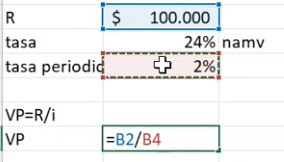
\includegraphics[trim=-5 -5 -5 -5 ,width=1\columnwidth]{8/Ejem8.png}} \\
  \multicolumn{3}{|c|}{\cellcolor[HTML]{FFB183}\textbf{5. Respuesta}}                         \\ \hline
  \multicolumn{3}{|p{\columnwidth}|}{
  El valor presente es VP = 5.000.000 COP
  }                                                                                           \\ \hline
  \multicolumn{3}{|c|}{\cellcolor[HTML]{FFB183}\textbf{6. Gráfica}}                           \\ \hline
  \multicolumn{3}{|c|}{No es necesaria una gráfica para este ejercicio.}                      \\ \hline
 \end{longtable}
 %\newline \newline %USARLO SI CREES QUE ES NECESARIO
\end{center}